\section{Computer Vision}\label{appendix:compvis}

Computer vision has its origins in the 1960s, when computer models were conceptualized in an attempt to simulate human perception. Back then, computer vision was studied following a "blocks" approach (polyhedra), as introduced by Larry Roberts \cite{huang1996computer}. Later, David Marr proposed a set of required stages for carrying out image understanding. His goal was to reach a 3D understanding of the models in a scene. Figure \ref{fig:marr-stages} illustrates Marr's algorithm to identify the visual world. 

\begin{figure}[!ht]
        \centering
        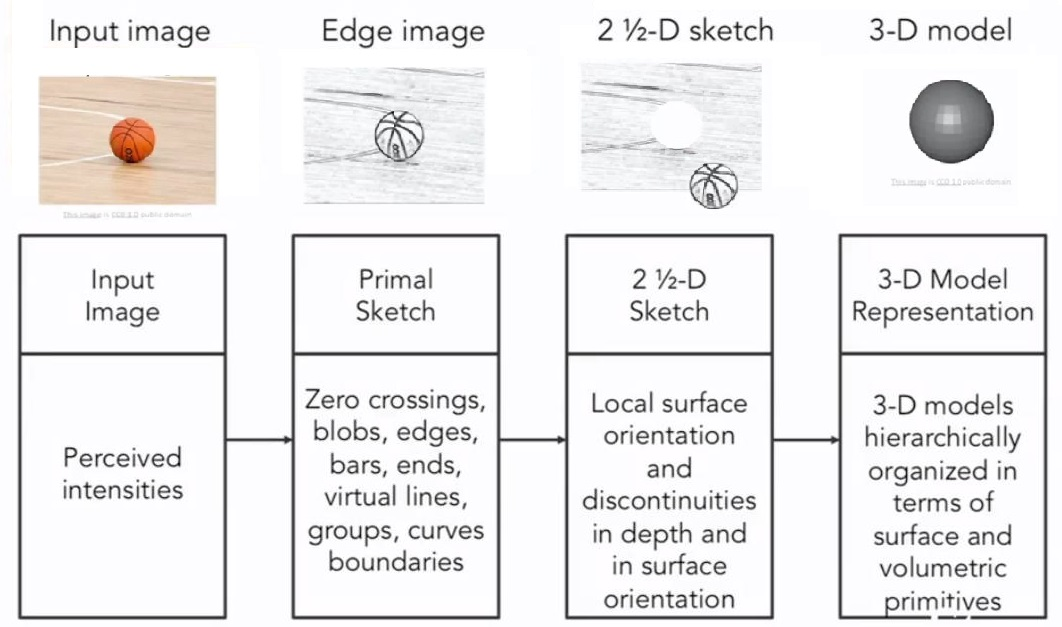
\includegraphics[width=0.72\textwidth]{images/marr-stages}
        \caption{David Marr's stages to identify the visual world.}
        \label{fig:marr-stages}
    \end{figure}
    
Throughout the years, however, most com\laeputer vision applications did not require complete 3D object models of the world. Nevertheless, Marr's paradigm shaped the future of computer vision for the years to come. The methods developed until circa 2000 analyzed images in terms of simple geometric features, such as a combination of lines.
% Most of the developed methods manipulated the pixels in images to create features.
The basic initial goal for computer vision was to achieve object segmentation, separating the background from salient objects. Later, the analysis of pixels and more complex features allowed to identify colors, shapes and objects in images. When the same features were seen in multiple images, an image could be classified by approximation. These collection of features for classification was called a "bag of words". Consequently, traditional machine learning approaches such as SVMs, boosting methods and graph models eased the usage of features for classification. Examples of features are:
\begin{itemize}
    \item Scale Invariant Feature Transform (SIFT) \cite{karami2017image}
    \item Speeded Up Robust Features (SURF) \cite{bay2006surf}
    \item Features from Accelerated Segment Test (FAST) \cite{rosten2006machine}
    \item Hough Transforms \cite{goldenshluger2004hough}
    \item Geometric Hashing \cite{tsai1994geometric}

\end{itemize}
Nowadays, traditional computer vision techniques are used in aerospace field, industrial automation, security inspections, intelligent transportation systems, security and transportation systems \citeauthor{bhargava2018fruits} are mostly used to perform simple tasks where machine learning is excessive or in situations where there are memory constraints (microcontrollers). However, machine learning methods for computer vision not only outperform classical computer vision in some tasks, but have also shown progress in classical computer-vision-dominated fields, such as embedded systems, as discussed by \textcite{zhang2019skynet} in \citetitle{zhang2019skynet}. 

%     \begin{itemize}
%         \item one paragraph of ML advancements 1960 - 2010
%         \item one paragraph how these methods are good at image processing but they showed lack of reliability without actually understanding what is in the scene
%     \end{itemize}

\subsection{Deep Learning for Vision}\label{appendix:DL-for-vision}
In 1943, following the ambition of trying to simulate the way the human brain is made up of a collection of simple units, McCulloch and Pitts \cite{mcculloch1943logical} developed a model of a neuron. They called this neuron MCP, which contributed to development of the neural networks we know today. Since around 2010, the rise of both public data and GPU hardware availability have allowed deep learning techniques to outperform traditional machine learning methods 
% deep learning, leveraged the computing power and data availability for training neural networks with many layers. 
% These deep neural networks can now outperform state of the art methods 
and reach super-human performance in a variety of tasks such as object detection, semantic segmentation, motion tracking, human pose estimation, and action recognition. 


\begin{figure}[!ht]
        \centering
        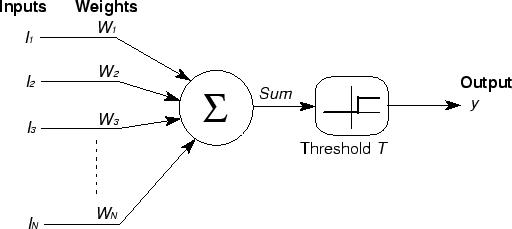
\includegraphics[width=0.5\textwidth]{images/mcculloch-pitts-model.png}
        \caption{McCulloch-Pitts model of a neuron.}
        \label{fig:mcculloch-neuron}
    \end{figure}


As of August 2021, ImageNet \cite{deng2009imagenet} has become one of the largest high-quality public databases for image classification and the paper \citetitle{krizhevsky2017imagenet} \cite{krizhevsky2017imagenet} has been cited over 85000 times. 
Other breakthroughs in the field, such as the alleviation of the vanishing gradients problem, new regularization techniques and the surge of frameworks for deep learning development, contributed to bringing machine and deep learning to the state we know of today.
% Finally, even though some fields have reached a level of maturity, such as 2D object detection, many tasks still have room for improvement. Nevertheless,
Consequently, deep learning techniques have defined themselves as the state-of-the-art for the task of object detection, which is of special interest for this work and further sections. 

% 3How Object Detection works
% Object detection can be performed using either traditional (1) image processing techniques or modern (2) deep learning networks.

% Image processing techniques generally don’t require historical data for training and are unsupervised in nature.
% Pro’s: Hence, those tasks do not require annotated images, where humans labeled data manually (for supervised training).
% Con’s: These techniques are restricted to multiple factors, such as complex scenarios (without unicolor background), occlusion (partially hidden objects), illumination and shadows, and clutter effect.
% Deep Learning methods generally depend on supervised training. The performance is limited by the computation power of GPUs that is rapidly increasing year by year.
% Pro’s: Deep learning object detection is significantly more robust to occlusion, complex scenes, and challenging illumination.
% Con’s: A huge amount of training data is required; the process of image annotation is labor-intensive and expensive. For example, labeling 500’000 images to train a custom DL object detection algorithm is considered a small dataset. However, many benchmark datasets (MS COCO, Caltech, KITTI, PASCAL VOC, V5) provide the availability of labeled data.


% Milestones in state-of-the-art Object Detection


% With the rise of CNNs, the foundation has been set for well-performing image classification approaches such as ResNet [6] or VGG [7]. In recent years, this development has gone even further towards systems which are capable of localizing or even masking out objects in images. Popular approaches with these capabilities are for example Mask R-CNN [9] or YOLO [8]. While using different approaches, both systems have the capability of localizing and semantically classifying objects in images. Mask R-CNN is even able to mask the pixel-areas that are belonging to the object by using polygonal shapes. In the background both approaches still rely on ResNet for feature extraction.

% While systems like these are highly impressive and sufficient for many cases, they are still far away from human visual perception and actual scene understanding [10]. Especially the shortcomings presented in section 1.2 apply to this kind of systems. The resulting polygon-masks or bounding boxes are not projected into 3D space but merely mapped onto the 2D coordinates of the image. If employed on sequential data, both systems would also need to reevaluate the whole frame on each timestep as they are not able to remember or track objects. This is problematic when understanding a scene, as it is often not likely for the whole scene to be visible at once, but only partially. Therefore we believe, it is crucial for a system not to forget but to accumulate information over timesteps.



% Most important two-stage object detection algorithms

% RCNN and SPPNet (2014)
% Fast RCNN and Faster RCNN (2015)
% Mask R-CNN (2017)
% Pyramid Networks/FPN (2017)
% G-RCNN (2021)
% Most important one-stage object detection algorithms

% YOLO (2016)
% SSD (2016)
% RetinaNet (2017)
% YOLOv3 (2018)
% YOLOv4 (2020)
% YOLOR (2021)

% Convolutional neural networks are a common approach to e .
% This section will briefly introduce two of the current state of the art methods for 2D object detection: Mask-RCNN and YOLO.
% (object segmentation). This section will add to the topic of semantic segmentation. 
% both 2D and 3D object detection attempt to
% Research on object segmentation has built upon the work done in previous image classification models to reach the current state of the art of 2D object segmentation: Mask R-CNN. The image saliency approach each (previous) model takes is described below:



\subsubsection{Object Detection}
Object detection involves localizing and classifying objects in a 2D image. Similarly, object segmentation is an extension of the recognition problem, which involves assigning labels to the specific pixels in a given image that belong to the detected objects. 

This section describes the problem of object detection as a way to infer semantics from the environment, which is an important concept for the later definition of semantic entropy in Chapter \ref{chap:3:title}. Methods for inferring semantics from the environment include:
\begin{itemize}
    \item Object Detection
    \item Object Segmentation
    \item Instance Segmentation
    \item Panoptic Segmentation
    \item Natural language descriptors of visual descriptors
\end{itemize}

Given the time constraint to experiment with different kinds of semantic entropy, this thesis will focus on 2D object detection methods for acquiring semantics from the environment. Therefore, two relevant algorithms will be described: Mask-RCNN and YOLO. For historical relevancy, 
% and completeness of this document, 
some traditional machine learning methods for 2D semantics are worth mentioning, such as: the Viola-Jones detector, HOG detectors, deformable part models, SVMs, Random Forests, K-means clustering. Deep learning architectures have however evolved extensively over the past few years and become the norm. Additionally:
\begin{itemize}
    \item Relevant two-stage detectors include: RCNN and SPPNet (2014), Fast RCNN and Faster RCNN (2015), Pyramid Networks/FPN (2017), G-RCNN (2021).
    \item Relevant one-stage object detection algorithms include: YOLO (2016), SSD (2016), RetinaNet (2017), YOLOv3 (2018), YOLOv4 (2020) and YOLOR (2021).
\end{itemize}

\begin{figure}[!ht]
        \centering
        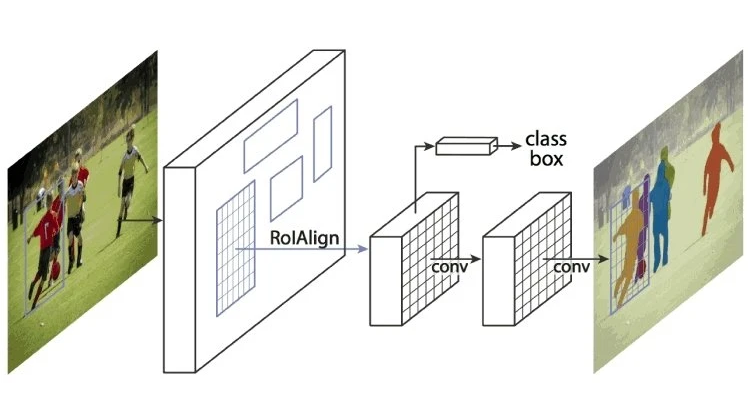
\includegraphics[width=0.5\textwidth]{images/maskrcnn.png}
        \caption{The Mask R-CNN Framework for Instance Segmentation \cite{visoai2021detection}.}
        \label{fig:maskrcnn}
    \end{figure}

\textbf{Mask-RCNN.}
Mask-RCNN's architecture (2017) is a two-stage object detector came to be as a sequential evolution of other architectures,
% , object segmentation techniques have tried to improve previous methods, 
% In Mask-RCNN's evolution since R-CNN, 
where previous iterations tackled given bottle necks to improve both accuracy and speed of the model. The first step in these detectors involves a region proposal method. The second step involves object classification and bounding box regression based on features obtained during previous step \cite{visoai2021detection}. The sequence of models that paved the road for Mask-RCNN are the following:
% The following methods have built upon the previous to reach state of the art performance:
\begin{itemize}
    \item \textbf{R-CNN:} a “selective search” algorithm proposes bounding boxes and features are obtained using a deep convolutional neural network (for example, AlexNet). Object classifications are then made with linear SVMs.
    \item \textbf{Fast R-CNN:} unifies the feature detector, and the bounding box predictor approach into a single model, but the region of interests are still part of the input. The shared computation showed speed improvements.
    \item \textbf{Faster R-CNN:} unifies the region proposal algorithm into the CNN model. This model merges a RPN (region proposal network) with Fast R-CNN.
    \item \textbf{Mask R-CNN:} extends the previous model to add pixel-level image segmentation. A small fully connected network was added that per region of interest outputs a segmentation mask.
\end{itemize}


\begin{figure}[!ht]
        \centering
        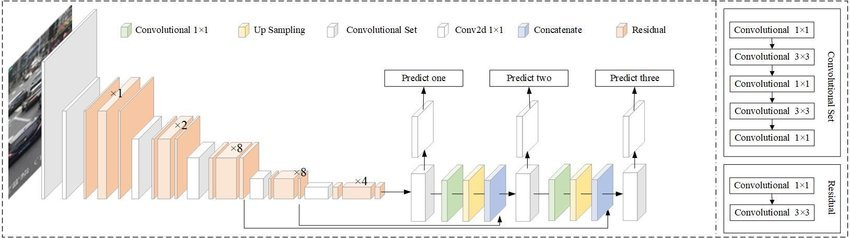
\includegraphics[width=0.8\textwidth]{images/yolov3.jpg}
        \caption{Structure detail of YOLOv3.It uses Darknet-53 as the backbone network and uses three scale predictions \cite{visoai2021detection}.}
        \label{fig:yolov3}
    \end{figure}
    
\textbf{YOLO.}
YOLO, in contrast, is a one-stage detection algorithm which directly predicts bounding boxes in a forward pass \cite{visoai2021detection}. This type of detectors tend to be faster and structurally simpler in exchange for less accuracy: YOLO is 1000x faster than R-CNN and 100x faster than Fast-RCNN. 
% Moreover, YOLOv3 achieves 57.9% 
% Understanding these basic overview of these approaches will prove useful for the pipeline this work proposes in the future chapters.
% The concept of semantics is of most interest here for our definition of uncertainty. 


YOLO, as shown in Figure \ref{fig:yolov3}, is a convolutional neural network which divides an input into cells or regions, and scores objects in these regions based on their similarity to predefined classes. For each region a set of anchor boxes is then predicted with a confidence score. Final boxes are then filtered via non-maximum suppression. Newer variants, such as YOLOv3 or YOLOv4 improve performance on smaller object, self-adversarial training and cross mini-batch normalization \cite{visoai2021detection}.

% maybe add a "whats next sentence"


% \section{Segmentation in 3D}
% % new
% https://www.synopsys.com/glossary/what-is-3d-image-segmentation.html
% https://arxiv.org/pdf/2103.05423.pdf
% https://www.octoconsulting.com/resource/3d-semantic-image-segmentation-real-world-applications-of-unreal-technology/
% https://igl.ethz.ch/projects/light-field-segmentation/


% \section{Recognizing Objects in 3D}
% what is 
% - https://arxiv.org/pdf/2010.15614.pdf
% what are benefits/ news
% https://www.socialmediatoday.com/news/google-has-developed-a-new-3d-object-recognition-process-which-could-lead/573965/
% - what are poses
% https://arxiv.org/pdf/2010.16279.pdf

\subsubsection{Pose Estimation in 3D}
Pose estimation is an extension of the 3D object recognition problem. It involves predicting a 3D translation and a 3D rotation. These types of methods have been trained using both synthetic \cite{gupta2015aligning} and real data \cite{li2019gs3d}, labeled with the 6D poses of the objects. Additionally, these methods can be 2D supervision-based or 3D supervision-based. 2D supervision-based methods utilize the information in the RGB image to predict a 3D bounding box, whereas 3D supervision-based methods directly detect 3D bounding boxes from stereo images, RGB-D cameras or LIDAR sensors \cite{sahin2020review}. 
\begin{figure}[!ht]
        \centering
        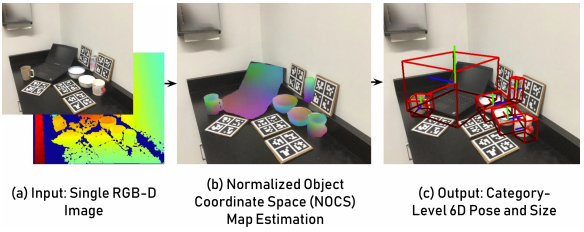
\includegraphics[width=0.7\textwidth]{images/wang-pose}
        \caption{Wang et al. proposed method for category-level 6D pose and
size estimation of multiple unseen objects in an RGB-D image.}
        \label{fig:wang-pose}
    \end{figure}
    
\textcite{sahin2020review} propose a discriminative categorization criteria to organize pose estimation techniques, as follows:
\begin{itemize}
    \item \textbf{Classification-based} approaches leverage 2D information to retrieve a 3D bounding box. Then, a refinement stage is added, such as random forests, to obtain the 6D pose of the object. Examples include: GS3D \cite{li2019gs3d}, Vote3Deep \cite{engelcke2017vote3deep} and the method by \textcite{michel2017global}.
    \item \textbf{Regression-based} approaches are similar to classification based approaches but they run another neural network directly over the predicted 3D bounding box to regress the 6D pose. Examples include: PointFusion \cite{xu2018pointfusion}, FusionNet \cite{hegde2016fusionnet}, VoxelNet \cite{zhou2018voxelnet}, AVOD net [108].
    \item \textbf{Classification and Regression-based} approaches run both tasks mentioned above under the same architecture. Examples include MonoPSR \cite{Ku_2019}, FrustumPNet \cite{qi2018frustum}, PointRCNN \cite{shi2019pointrcnn}, SSD-6D \cite{kehl2017ssd} and DeepContext \cite{zhang2017deepcontext}.
    \item \textbf{Template matching} approaches look at an image using sliding windows and compare obtained features with a database of pre-defined feature templates, and the pose parameter is given to the window with the closest similarity to the template matched. Examples include: the LINEMOD adaptation from \textcite{hinterstoisser2012model}, SVMs embedded in Adaboost \cite{rios2013discriminatively}, RAPID-LR \cite{Munoz_2016} and the method proposed by \textcite{Ku_2018}.
    \item \textbf{Point-pair feature matching} approaches were proposed by \textcite{drost2010model}. The idea is to store point-pair features in a hash table in a separate "offline" stage. During prediction, potential matches then are obtained by comparing to a global model representation. Finally, these matches vote on the pose parameters. These methods underperform given objects with similar features, occlusion and sensor noise \cite{Mohamad_2014}. 
    \end{itemize}


    
Unfortunately, the limitations and challenges mentioned in section \ref{chap:2:3d} overlap with the ones from pose estimation. Along these lines, work by \textcite{Wang_2019} attempts to push pose estimation techniques to being able to generalize to unknown objects, removing the dependency to knowing an object's 3D model previously. Figure \ref{fig:wang-pose} illustrates a glimpse to the method proposed by Wang et al.


% \lipsum[1-3]

    % \begin{itemize}
    %     \item one paragraph of rise of CNNs 2010 - present
    %     \item one paragraph how these methods are not enough for 3d space yet, and importance of not forgetting over timesteps
    % \end{itemize}



    % \begin{itemize}
    %     \item one paragraph about cow robot milking industry
    %     \item ??
    %     \item one paragraph about cow teat morphology 
    % \end{itemize}
% \section{Summary}\label{chap:2:summary}
% % half a page
% \lipsum[1-2]

    % \begin{itemize}
    %     \item one paragraph: describe popular approaches briefly, and main ways literature does it
    %     \item 1P: highlight most interesting literature approach
    %     \item 1P: lastly, we discuss how X is done, and whether it is feasible to extend our approach (prob a small filler?)
    % \end{itemize}
% new

\subsubsection{3D Methods}

\textcite{han2019image} provide a thorough review of recent research for 3D object reconstruction. 

A brief overview of the methods that have been successful at 3D object recognition and reconstruction is presented below:
\begin{itemize}

    \item The majority of works pre-2018 use voxelized representations \cite{yan2016perspective} \cite{choy20163d} \cite{wu2016learning}, which allow the representation of arbitrary topology considering both the surface and the internal structure of object. Representation types of data are: volumetric (based on 3D voxel grids), surface-based (meshes, point clouds) and intermediate (3D reconstruction is done based off 2D information from RGB images).
    \item Since convolutions and overall processing of 3D images has a high memory requirement, volumetric techniques leverage octrees \cite{meagher1980octree}, which are sparse partitioning techniques for 3D grid structures (O-CNN \cite{wang2017cnn}, OGN \cite{tatarchenko2017octree}, OctNet \cite{riegler2017octnet}) to achieve high resolutions while maintaining memory efficiency. As described by \textcite{tatarchenko2017octree}, Octree Generating Networks reduce memory requirements for reconstruction from 4.5 GB to 0.29 GB. These techniques, however, are complex to implement which impacts their reproducibility and further research.
    \item Other approaches learn continuous Signed Distance Functions \cite{park2019deepsdf, chen2019learning} or continuous occupancy grids \cite{mescheder2019occupancy}. These methods have a lower memory requirement and can reconstruct the 3D object at the desired resolution. 
    \item Methods that look at multiple frames for reconstructing representations outperform single-view methods for they collect more information about the silhouette of the objects. 
    \item Techniques that try to reconstruct primarily the surface of a seen object (surface-based techniques) outperform volumetric methods by a small margin. These are: Mesh-based approaches \cite{pontes2018image2mesh} and Point-based approaches \cite{kurenkov2018deformnet, fan2017point}.
    \item Methods that utilize 2D supervision to reconstruct 3D objects improved their performance since 2017, and are outperformed by 3D supervision-based approaches by a small margin. \cite{yan2016perspective, arsalan2017synthesizing}.
\end{itemize} 

Similarly, \citeauthor{han2019image} provide a set of research directions based on the challenges and limitations that 3D object recognition currently faces. These areas of improvement can be summarized as follows:
\begin{itemize}
    \item Bigger training data sets since deep learning methods depend heavily on them. 
    \item Generalization to unseen objects, and not just specific-domain models.
    \item Methods that allow for 3D reconstruction in higher resolutions, such as reconstruction of hairs, fur and plants.
    \item Combined approaches for both recognition and reconstruction in a single method.
    \item Domain specialized methods that can perform well also on unseen objects, but of a specific domain, say wild animals, which are not easy to label.
    \item Reconstruction of 3D video streams where frames are missing and information is passed from future frames to previous ones.
    \item Full 3D scene understanding, which requires detection, recognition, reconstruction, spatial awareness and robustness to unseen objects.
\end{itemize}

% \begin{figure}[!ht]
%         \centering
%         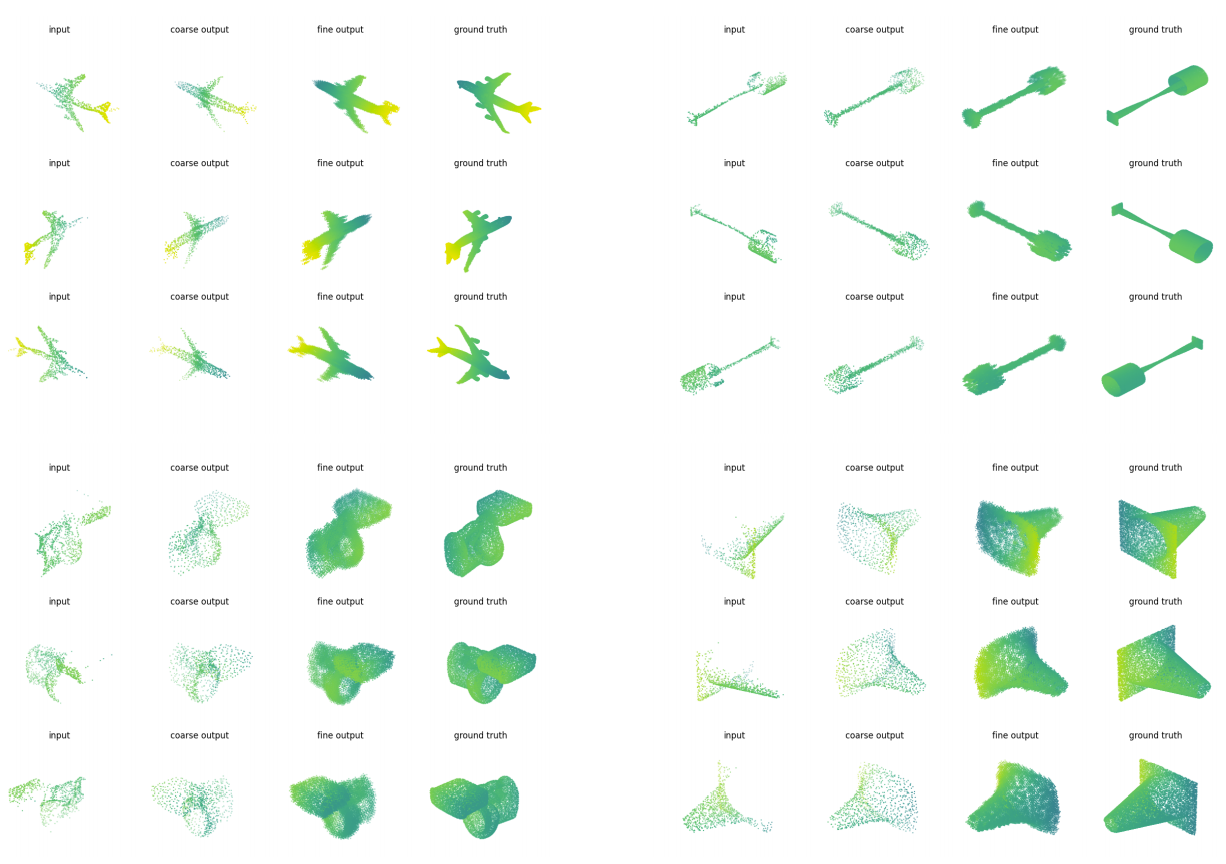
\includegraphics[width=0.8\textwidth]{images/occo-results}
%         \caption{Results of using OcCo (2020) pre-training for completion of point clouds.}
%         \label{fig:occo-results}
%     \end{figure}
    
% new


% \section{Synthetic Dataset Generation Overview}
% \label{appendix:ndds}

% \begin{figure}[!ht]
%     \centering
%     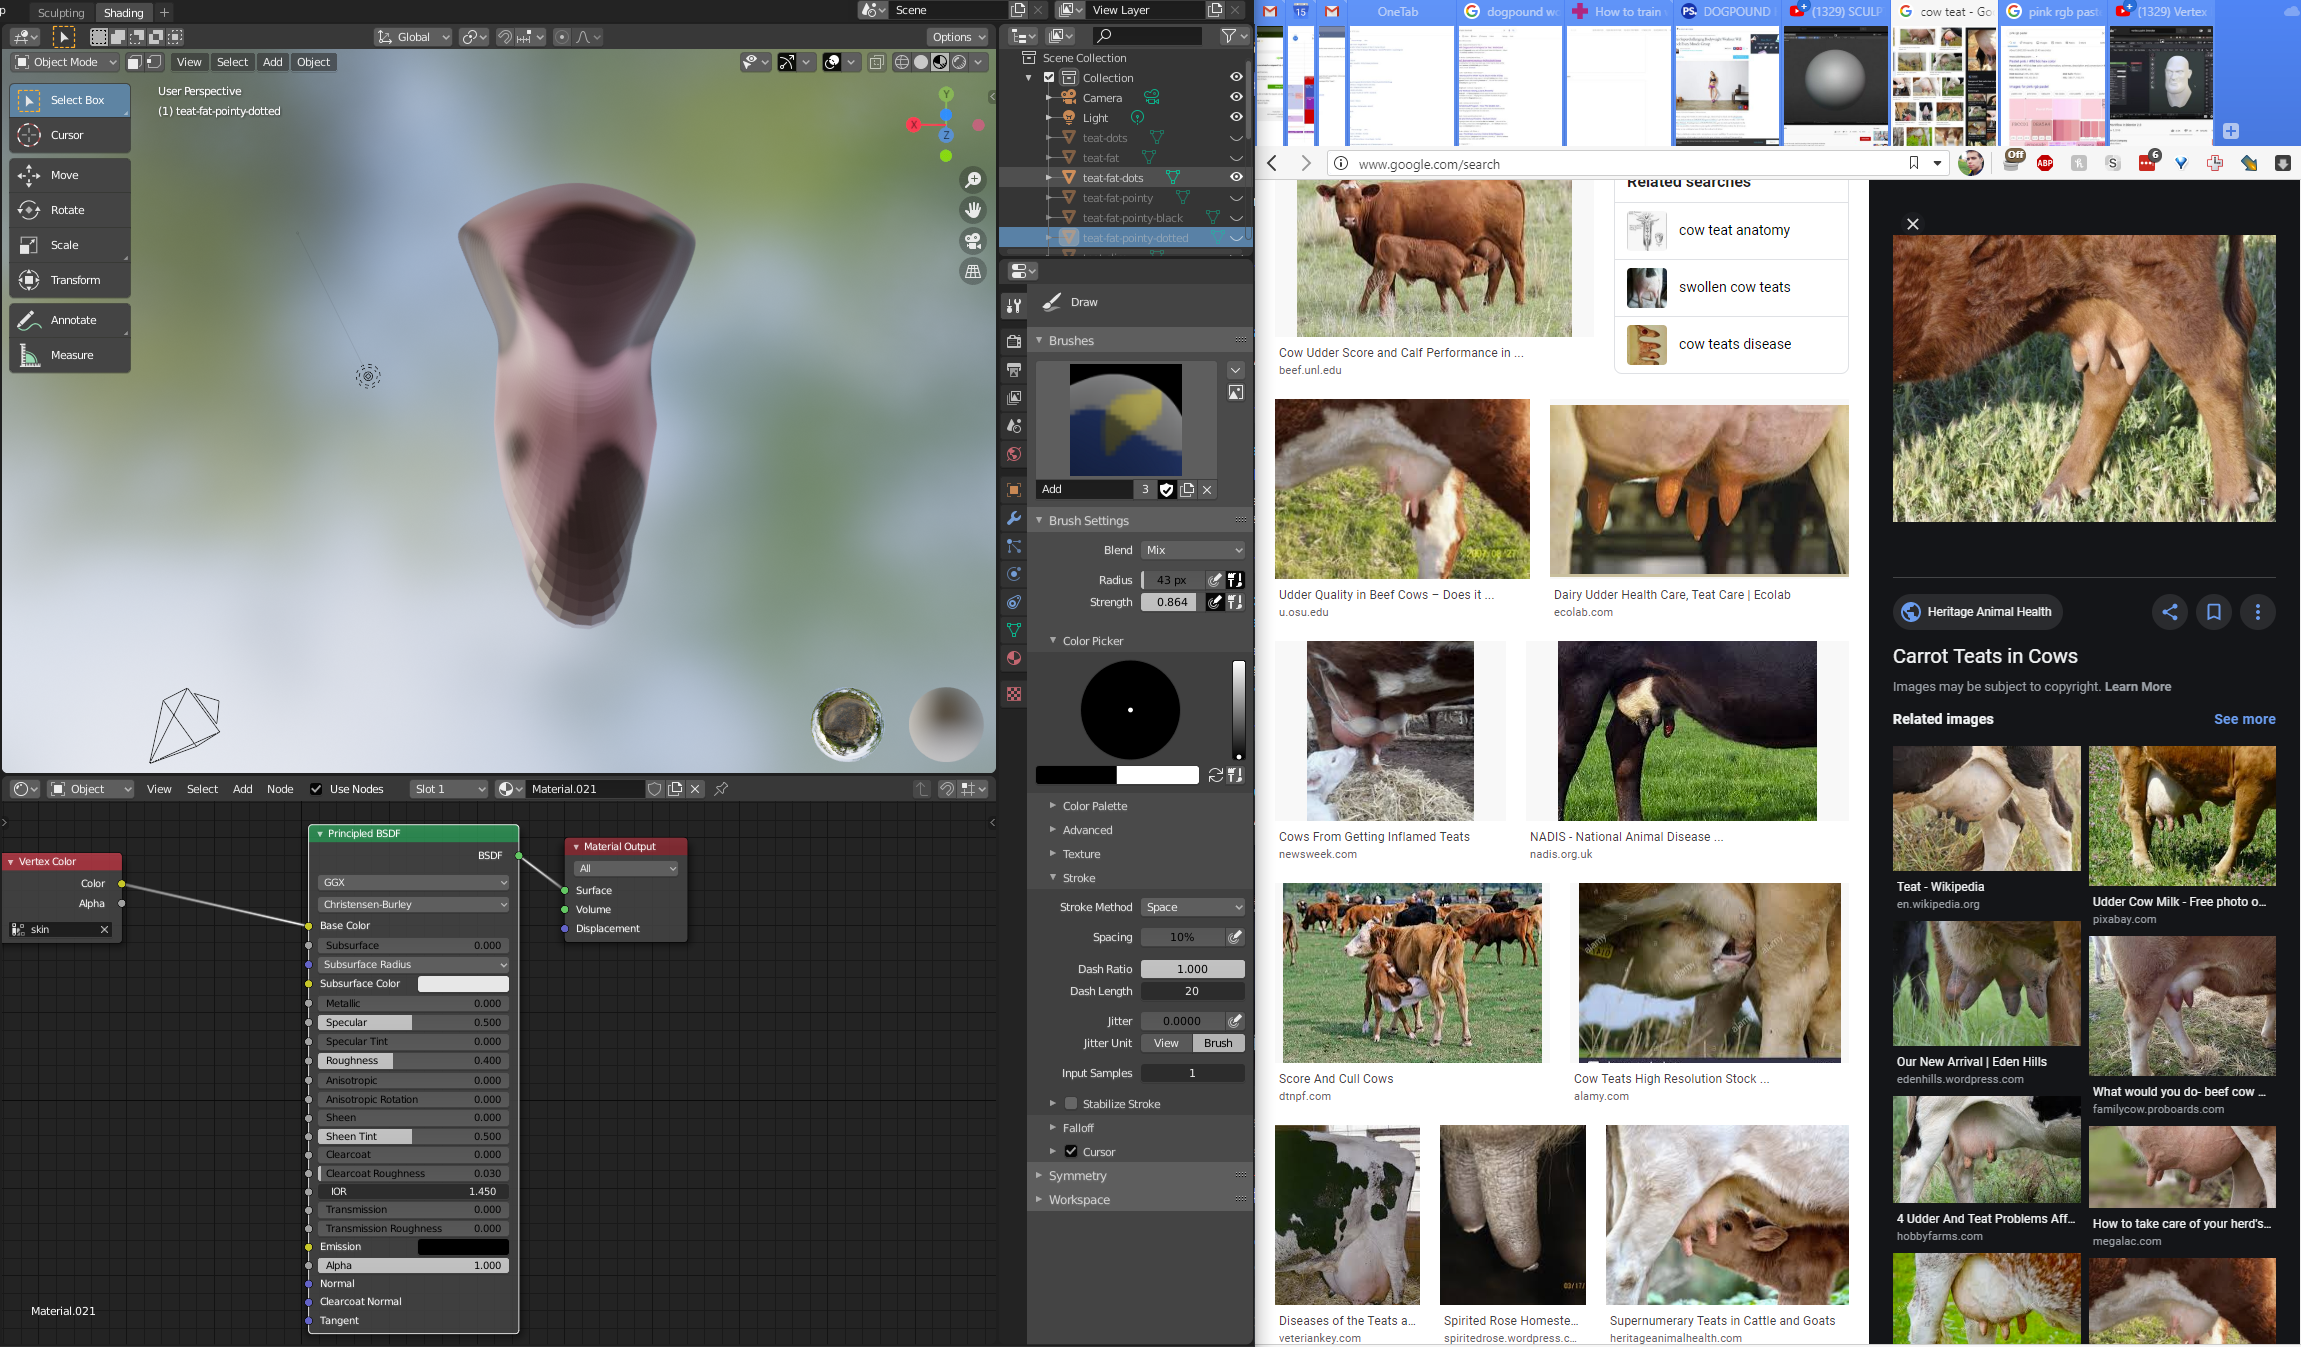
\includegraphics[width=.8\textwidth]{images/ndds1}
%     \caption{Screenshot of a photorealistic scene in Unreal Engine 4.}
%     \label{fig:ue4-1}
% \end{figure}
% \begin{figure}[!ht]
%     \centering
%     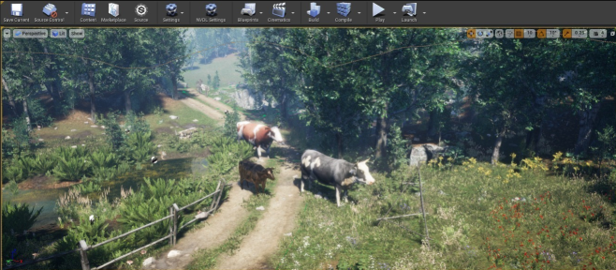
\includegraphics[width=.8\textwidth]{images/ndds2}
%     \caption{Screenshot of a photorealistic scene in Unreal Engine 4.}
%     \label{fig:ue4-2}
% \end{figure}
% \begin{figure}[!ht]
%     \centering
%     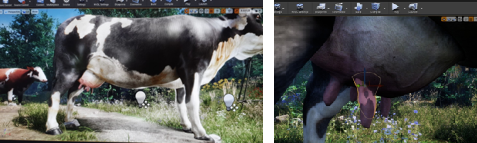
\includegraphics[width=0.8\textwidth]{images/ndds3}
%     \caption{Screenshot of a photorealistic scene in Unreal Engine 4.}
%     \label{fig:ue4-3}
% \end{figure}
% % \begin{figure}[!ht]
% %     \centering
% %     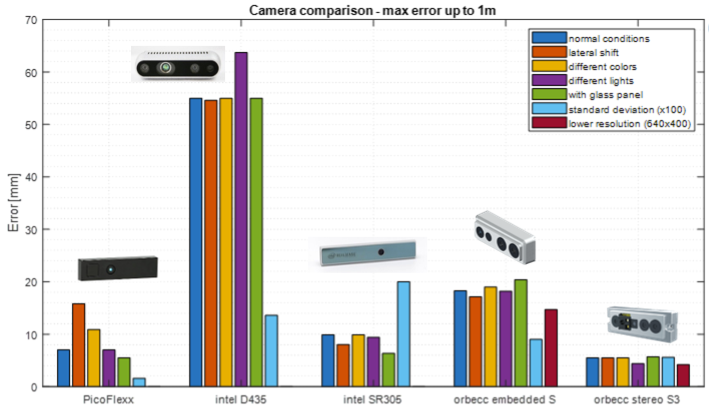
\includegraphics[width=1\textwidth]{images/camera_choice.png}
% %     \caption{Screenshot of a sample export from the NDDS plugin.}
% %     \label{fig:ndds}
% % \end{figure}

% \newpage
% \section{Pose Estimation Processing Pipeline}
% \label{appendix:cow_design}
% \begin{figure}[!ht]
%     \centering
%     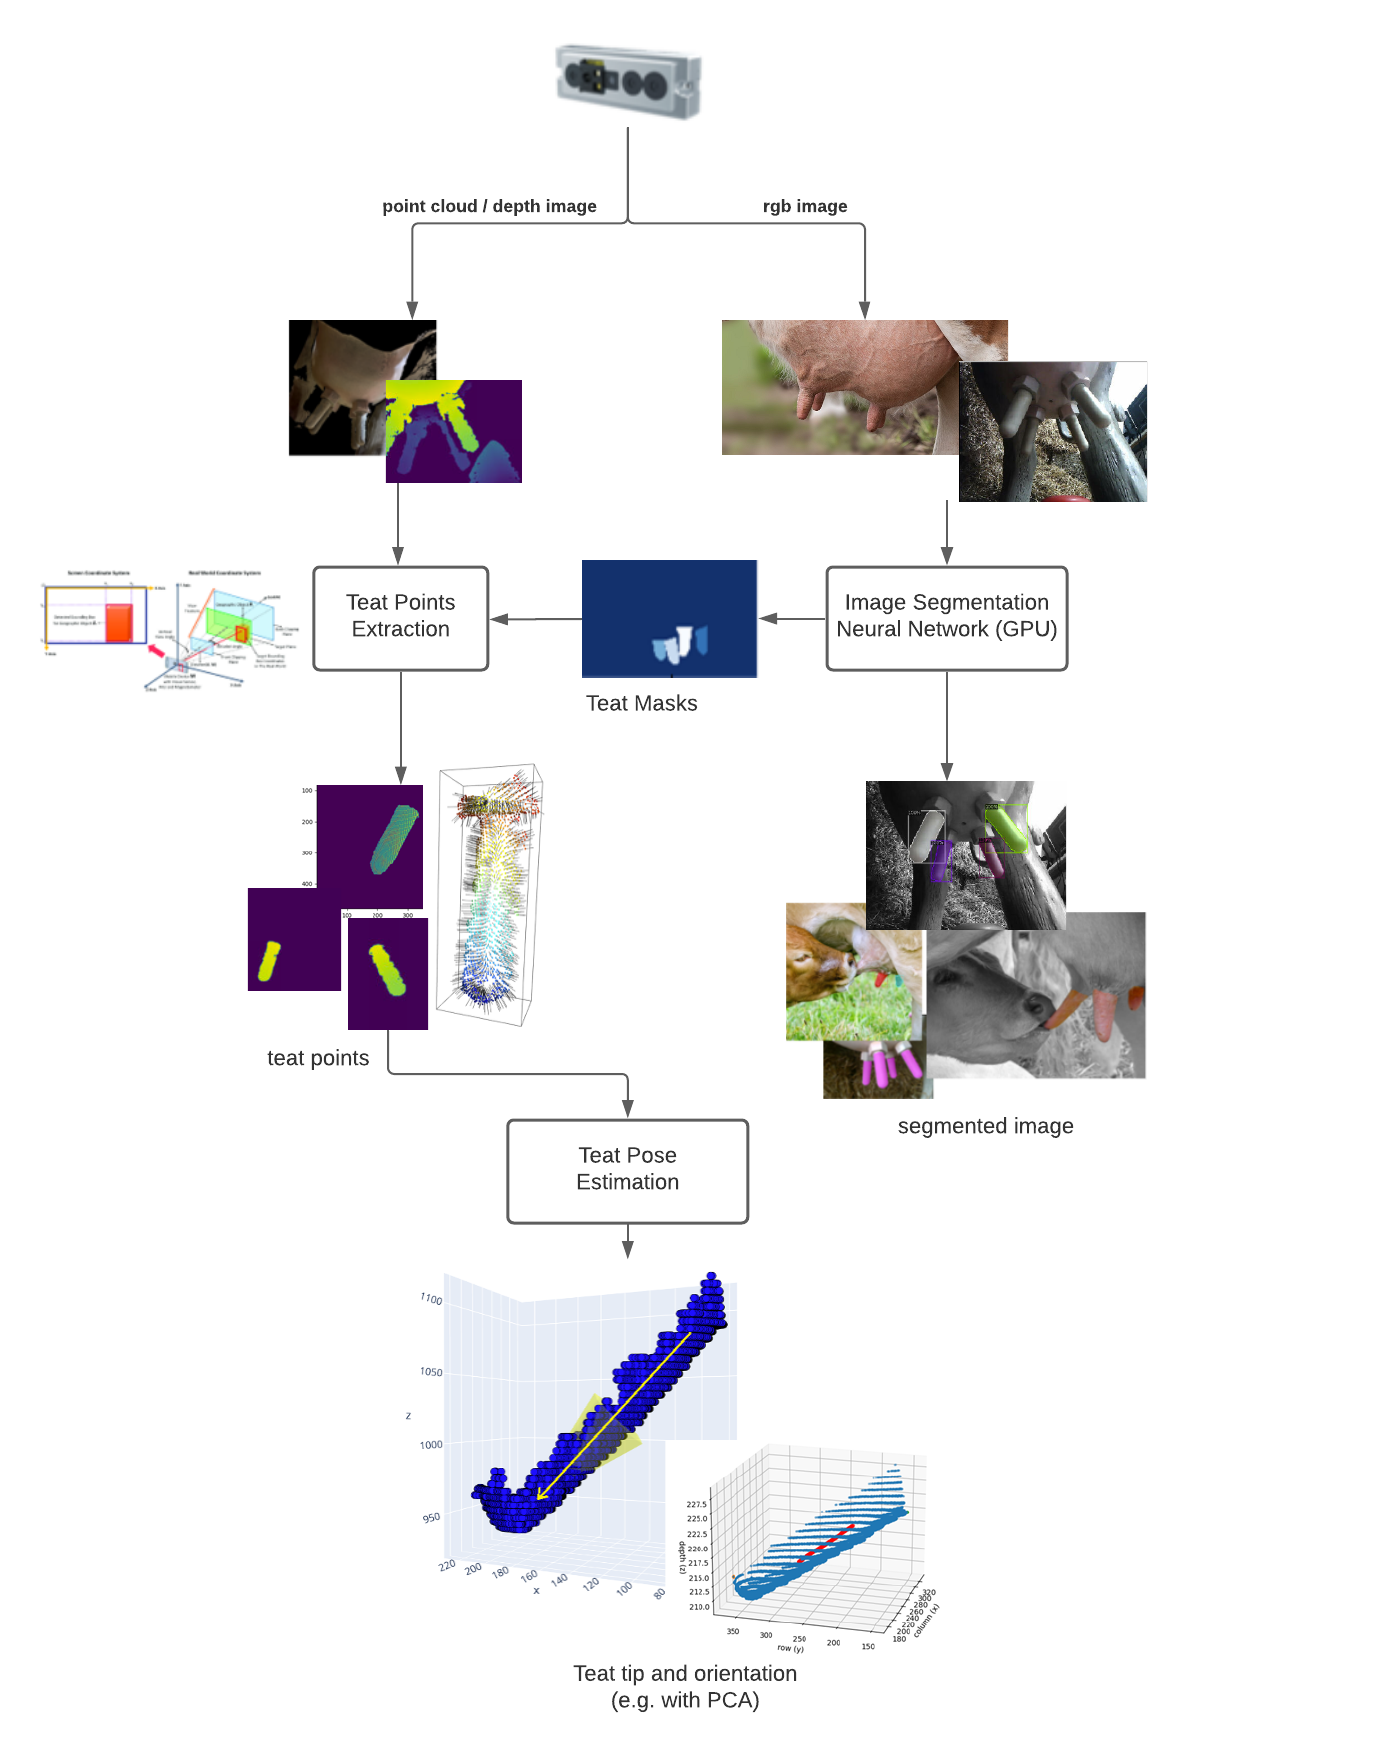
\includegraphics[width=1\textwidth]{images/cow_design.png}
%     \caption{Pose Estimation Processing Pipeline Flowchart}
%     \label{fig:cow_design}
% \end{figure}

% \newpage
% \section{Camera Evaluation}
% \label{appendix:camera_evaluation}

% \begin{figure}[h]
%         \centering
%         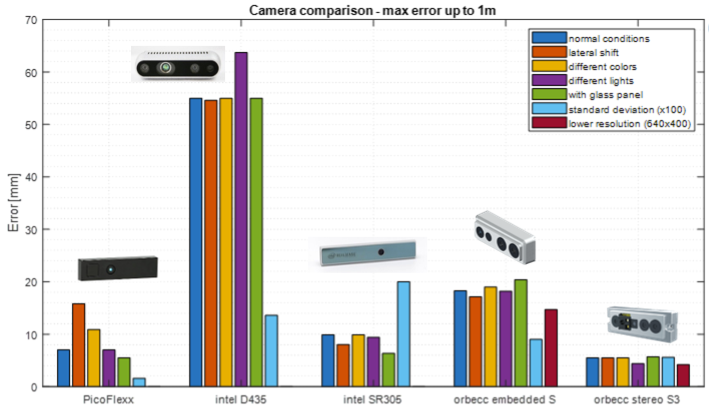
\includegraphics[width=0.8\textwidth]{images/camera_choice.png}
%         \caption{Camera Performance Evaluation}
%         \label{fig:camera_choice}
%     \end{figure}
  
  
  
% \newpage
% \section{Pose Estimation Error Correlogram}  
% \label{appendix:correlogram}
% \begin{figure}[h]
%         \centering
%         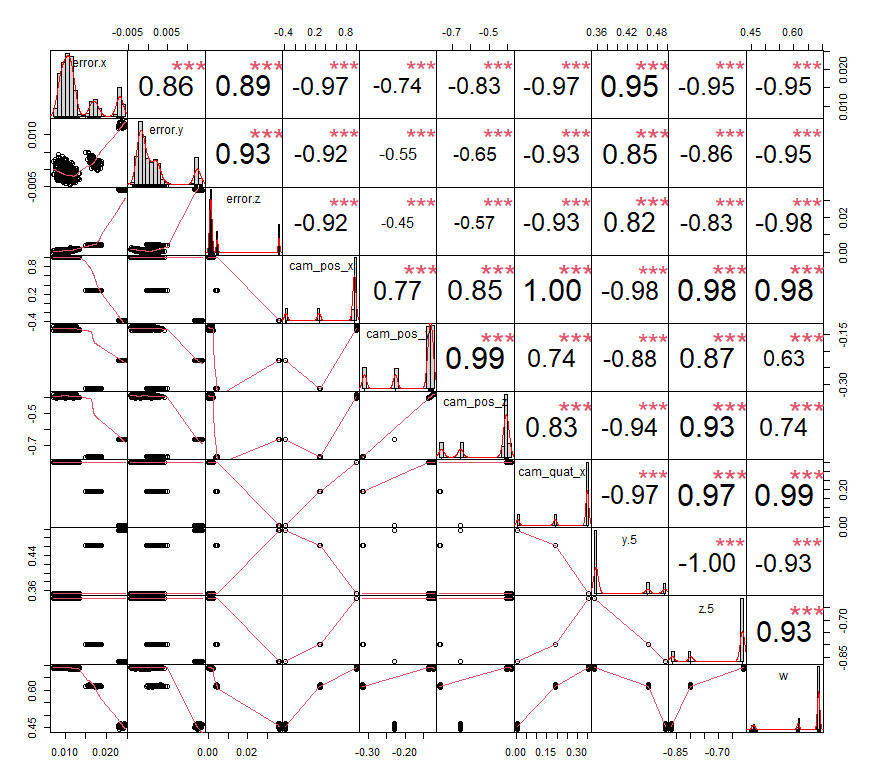
\includegraphics[width=0.9\textwidth]{images/r_correlogram.png}
%         \caption{Correlogram of the errors in (x, y, z) and the camera position variables (x, y, z, quaternion) for the MAV algorithm.}
%         \label{fig:correlogram}
% \end{figure}

